\chapter{Acoustic emissions}

Modeling the acoustic emissions is a core feature of APECSS. To this end, APECSS offers different models for the acoustic emissions, assuming an incompressible liquid, a weakly-compressible liquid or a fully-compressible liquid. To account for a finite propogation speed, the information associated with an emitted acoustic wave is propagated along the radial coordinate axis using a Lagrangian wave tracking approach.

\vspace{0.8em}

\noindent
\begin{tabular}{p{0.12\textwidth} p{0.32\textwidth} p{0.45\textwidth}}
    \textbf{Section} &\textbf{Command} & \textbf{Description} 
\vspace{1mm} \\ \hline
{\tt BUBBLE} & {\tt Emissions Incompressible} & Computes the acoustic emissions under the common incompressible assumption.\\ 
& {\tt Emissions FTI} & Computes the acoustic emissions under the assumption of an incompressible fluid but propagating the emissions with the speed of sound.\\ 
& {\tt Emissions QA} & Computes the acoustic emissions using the quasi-acoustic model of \citet{Gilmore1952}.\\ 
& {\tt Emissions KB} & Computes the acoustic emissions based on the Kirkwood-Bethe hypothesis.\\ 
 \hline
\end{tabular} \vspace{1em}

\section{Lagrangian wave tracking}

APECSS tracks acoustic emissions using a Lagrangian wave tracking approach, illustrated in Figure \ref{fig:lagrangiantracking}, in which so-called \textit{emission nodes} are propagated in the radial direction with propagation speed $\mathcal{C}$. Each emission node, represented in APECSS as a structure {\tt struct APECSS\_EmissionNode} and part of a linked list of these structures, holds the current radial coordinate $r(t)$, the flow velocity $u(r,t)$, the pressure $p(r,t$), the enthalpy $h(r,t)$ if applicable, as well as the invariants $f(\tau)$ and $g(\tau)$ computed based on the solution of the RP model. The definition of the propagation speed $\mathcal{C}$ depends on the chosen model.

The radial position of an emission node at time $t$ is given as
\begin{equation}
    r(t) = R(\tau) + \int_\tau^t \mathcal{C} \, \mathrm{d}t \approx R(\tau) + \sum_{i=1}^N \mathcal{C}(r(t_{i}),t_{i})  \, \Delta t_{i}, 
    \label{eq:r_t}
\end{equation}
where $\Delta t$ is the numerical time-step and $N$ is the number of time-steps making up the time interval from $\tau$ to $t$. 

\begin{figure}
    \begin{center}
    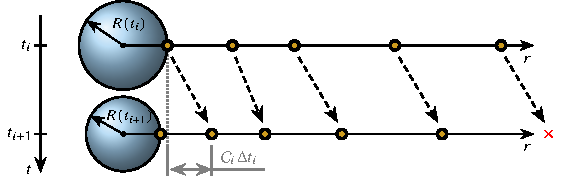
\includegraphics[width=0.7\linewidth]{LagrangianWaveTracking.pdf}
    \caption{Illustration of the Lagrangian transport of the emission nodes, updated at each discrete time instance $t_i$. Nodes that pass a predefined maximum radial coordinate are discarded.}
    \label{fig:lagrangiantracking}
    \end{center}
\end{figure}

\section{Incompressible assumption}

Assuming an incompressible liquid ($c_{\ell,\mathrm{ref}} \rightarrow  \infty$) with density $\rho_{\ell,\mathrm{ref}}$, the velocity $u(r,t)$ and pressure $p(r,t)$ at a given radial location $r(t)$ are defined as \citep{Neppiras1980}
\begin{equation}
    u(r,t) = \frac{R(t)^2 \dot{R}(t)}{r^2}  \label{eq:u_rt_incomp} 
\end{equation}
and 
\begin{equation}
    p(r,t) = p_\infty(t) + \rho_{\ell,\mathrm{ref}} \left[\frac{R(t)^2 \, \ddot{R}(t) + 2 \, R(t) \, \dot{R}(t)^2}{r} - \frac{R(t)^4 \, \dot{R}(t)^2}{2 \, r^4} \right], \label{eq:p_rt_incomp}
\end{equation}
respectively. The assumption of an incompressible fluid is consistent with the Rayleigh-Plesset models in Eqs.~\eqref{eq:standardRP} and \eqref{eq:modRP}. Note that, because $\mathcal{C} \rightarrow \infty$, these simple incompressible acoustic emissions do not use the Lagrangian wave tracking and no emission nodes are defined and processed, since pressure and velocity are defined instantaneously for all $r$.

Alternatively, APECSS also supports the assumption that the liquid is incompressible but the information associated with the acoustic emissions still propagates with finite speed $\mathcal{C} = c_{\ell,\mathrm{ref}}$ using the Lagrangian wave tracking approach.  This approach, referred to in APECSS as {\tt FTI} or \text{finite-time incompressible}, accurately recovers the time delay between emitting information and this information arriving in a certain location.

\section{Quasi-acoustic model}
\label{sec:emissionsqa}

Assuming the liquid is compressible but accurately described by a constant density $\rho_{\ell,\mathrm{ref}}$ and constant speed of sound $c_{\ell,\mathrm{ref}}$, \citet{Gilmore1952} derived the {\it quasi-acoustic model} for the acoustic emissions. With the quasi-acoustic model, the velocity, pressure and radial location follows as
\begin{align}
    u(r,t) &= \frac{f(\tau)}{r(t)^2} + \frac{g(\tau)}{r(t) \, c_{\ell,\mathrm{ref}}}  \label{eq:u_rt_qa} \\
  p(r,t) &=  p_\infty(t) + \rho_{\ell,\mathrm{ref}} \left[ \frac{g(\tau)}{r(t)} - \frac{u(r,t)^2}{2} \right] \label{eq:p_rt_qa} \\
  r(t) &\approx R(\tau) + c_{\ell,\mathrm{ref}} \sum_{i=1}^N \Delta t_{i-1}, \label{eq:r_t_qa}
\end{align}
where $f(\tau)$ and $g(\tau)$ are invariants defined based on the result of the employed RP model as
\begin{align}
    f(\tau) &= R(\tau)^2 \dot{R}(\tau) - \frac{R(\tau) g(\tau)}{c_{\ell,\mathrm{ref}}}\\
    g(\tau) &= R(\tau) \left[\frac{p_\mathrm{L}(\tau)-p_\infty}{\rho_{\ell,\mathrm{ref}}} + \frac{\dot{R}(\tau)^2}{2} \right],
\end{align}
and $\tau$ is the time at which the acoustic wave is emitted at the bubble wall. For $t=\tau$ with $r=R(\tau)$, Eq.~(\ref{eq:u_rt_qa}) reduces to $u(R,\tau)=\dot{R}(\tau)$ and Eq.~(\ref{eq:p_rt_qa}) reduces to $p(R,\tau)=p_\mathrm{L}(\tau)$, thus satisfying the boundary conditions at the bubble wall. 

The quasi-acoustic model is consistent in its modelling assumptions with the Keller-Miksis model, Eq.~\eqref{eq:keller}. The applicability of the quasi-acoustic model is limited to small Mach numbers, $(\dot{R}/c_0)^2 \ll 1$, as it incorporates a finite propagation speed of the acoustic emissions and the nonlinear pressure contributions resulting from the flow, but since all parts of the wave propagate with speed $c_0$, the quasi-acoustic model can neither describe the nonlinear distortion of acoustic waves nor the formation of shock fronts. 

\section{Emissions based on the Kirkwood-Bethe hypothesis}
\label{sec:emissionskb}

Following a similar derivation as for the quasi-acoustic model presented in Section \ref{sec:emissionsqa}, but assuming a fully compressible liquid described by a suitable equation of state, a model for the acoustic emissions based on the Kirkwood-Bethe hypothesis \citep{Kirkwood1942,Cole1948} can be derived. The velocity, enthalpy and radial location of an emission node are then given as
\begin{align}
    u(r,t) &= \frac{f(\tau)}{r(t)^2} + \frac{g(\tau)}{r(t) \, [c(r,t) + u(r,t)]}  \label{eq:u_rt_kb} \\
    h(r,t) &= h_\infty(t) + \frac{g(\tau)}{r(t)} - \frac{u(r,t)^2}{2}. \label{eq:h_rt_kb}\\
    r(t) &\approx R(\tau) + \sum_{i=1}^N \big[c(r(t_i),t_i) + u(r(t_i),t_i) \big] \Delta t_{i}, \label{eq:r_t_kb}
\end{align}
where $\tau$ is the time at which the acoustic wave is emitted at the bubble wall.
The invariants $f(\tau)$ and $g(\tau)$ are defined as
\begin{align}
    f(\tau) &= R(\tau)^2 \dot{R}(\tau) - \frac{R(\tau) \, g(\tau)}{c_\mathrm{L}(\tau) + \dot{R}(\tau)}   \label{eq:f_R} \\  
    g(\tau) &= R(\tau) \left[h_\mathrm{L}(\tau) - h_\infty(\tau) + \frac{\dot{R}(\tau)^2}{2} \right]
    \label{eq:g_R} ,
\end{align}
For $t=\tau$ with $r=R(\tau)$, Eq.~(\ref{eq:u_rt_kb}) reduces to $u(R,\tau)=\dot{R}(\tau)$ and Eq.~(\ref{eq:h_rt_kb}) reduces to $h(R,\tau)=h_\mathrm{L}(\tau)$, thus satisfying the boundary conditions at the bubble wall. The pressure $p(r,t)$ can then be readily computed based on the employed equation of state from the enthalpy $h(r,t)$. The assumptions used to derive this model for the acoustic emissions are consistent with the Gilmore model, Eq.~\eqref{eq:gilmore}.

Emission nodes with a higher pressure propagate faster than nodes with a lower pressure, which in turn leads to progressive steepening of the acoustic wave. As a result, an emission node may overtake the forerunning emission node, yielding an unphysical multivalued solution. In reality, such a multivalued solution is avoided by the formation of a shock front \citep{Fay1931}. \citet{Rudnick1952} postulated that the rate of attenuation of a stable shock front is independent of the dissipation process leading to the stable shock front. Exploiting Rudnick's argument, an emission node that overtakes its forerunning neighbor is simply discarded, see Fig.~\ref{fig:lagrangiantrackingshock}, thus maintaining a physically plausible solution.

\begin{figure}
    \begin{center}
    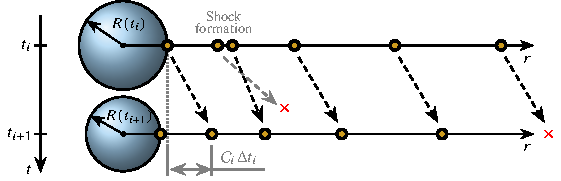
\includegraphics[width=0.7\linewidth]{LagrangianWaveTracking_withShock.pdf}
    \caption{Illustration of the Lagrangian transport of the emission nodes, updated at each discrete time instance $t_i$. Nodes that either overtake the forerunning node, which represents the formation of a shock front, or that pass a predefined maximum radial coordinate are discarded.}
    \label{fig:lagrangiantrackingshock}
    \end{center}
\end{figure}


\section{Results}

APECSS can write out different results based on the acoustic emissions. Note that APECSS does \underline{not} write any results to disk unless it is specifically ask to do so.

The acoustic emissions can be recorded as a function of time at one or multiple radial locations (cf.~{\tt EmissionsSpace}), or the emissions are written out with respect to their radial location at one or multiple time instances (cf.~{\tt EmissionsTime}), for one or multile specific emission nodes (cf.~{\tt EmissionsNode}) or for selected extrema in a specified period (cf.~{\tt EmissionsMinMax}). This calls can be used multiple times to defined, for instance, multiple radial locations or time instances.

\vspace{0.8em}

\noindent
\begin{tabular}{p{0.1\textwidth} p{0.36\textwidth} p{0.49\textwidth}}
    \textbf{Section} &\textbf{Command} & \textbf{Description} 
\vspace{1mm} \\ \hline
{\tt RESULTS} & {\tt OutputPath <string>} & Path to the directory where all the results should be written in to (default: {\tt ./}).\\
& {\tt OutputDigits <int>} & Results are written out with as many digits (default: 6).\\
& {\tt EmissionsSpace <float>} & Defines a radial location at which the emissions in the liquid are written out as a function of time. If/while the location is in the gas phase, $0$ is recorded.\\ 
& {\tt OutputFreqEmissionsSpace <int>} & Results of the emissions at a specific radial location are stored every so many time steps (default: 1).\\ 
& {\tt EmissionsTime <float>} & Defines a time instance at which the emission in the liquid are written out as a function of the radial coordinate.\\ 
& {\tt EmissionsNode <int>} & Defines a node ID of which the emission in the liquid are written out as a function of the radial coordinate.\\ 
& {\tt EmissionsMinMax <int>} & Defines the period in which the emission in the liquid are written out as a function of the radial coordinate for the node representing $R_\mathrm{min}$, $\dot{R}_\mathrm{min}$ and $p_\mathrm{L,max}$.\\ 
 \hline
\end{tabular} \vspace{1em}